\begin{frame}{Коммуникационные протоколы. $f: X \times Y \to \mathcal{O}$}
    \begin{center}
    	\onslide<1->{
    \tikzstyle{op1} = [opacity = 0]
    \tikzstyle{op2} = [opacity = 0]
    \tikzstyle{op3} = [opacity = 0]
    \tikzstyle{op4} = [opacity = 0]
}
\only<2->{\tikzstyle{op2} = [opacity = 1]}
\only<3->{\tikzstyle{op3} = [opacity = 1]}
\only<4->{\tikzstyle{op4} = [opacity = 1]}

\begin{tikzpicture}[>=latex]
    \node (alice) at (0, 0) {\includegraphics[scale = 0.15]{pics/utia-food-1.png}};
    \node (bob) at (7, 0) {\includegraphics[scale = 0.15]{pics/utia-food-2.png}};
    \node[above = 0.3 of alice] {$x \in U$};
    \node[above = 0.3 of bob] {$y \in V$};

    \path (alice.east) -- (bob.west) node[midway, above = 2.3] {\Large $f(x, y) = ?$};
    \draw[op2, ->, thick] ($(alice.east) + (0.3, 1)$) -- ($(bob.west) + (-0.3, 1)$) node[midway, above]
        {$r_1 = a(x)$};
    \draw[op3, <-, thick] ($(alice.east) + (0.3, 0.2)$) -- ($(bob.west) + (-0.3, 0.2)$)
        node[midway, above] {$r_2 = b(y, r_1)$};
    \draw[op4, ->, thick] ($(alice.east) + (0.3, -0.2)$) -- ($(bob.west) + (-0.3, -0.2)$);
    \draw[op4, ->, thick] ($(alice.east) + (0.3, -0.6)$) -- ($(bob.west) + (-0.3, -0.6)$)
        node[midway, below] {$\vdots$}; 
\end{tikzpicture}    
    \end{center}

    \pause
    \pause
    \pause
	\pause
    
    Глубина коммуникационного протокола~--- число раундов в худшем случае.
    
    $\CC(f)$~--- минимальная глубина коммуникационного прокола для функции $f$.
\end{frame}

\begin{frame}{Протоколы и деревья}

    Алиса получает $x \in X$, а Боб получает $y \in Y$. Коммуникационный протокол соответствует дереву:
    \begin{columns}[t]
		\begin{column}{0.7\textwidth}
            \begin{itemize}
                \item<2-> внутренние вершины помечены игроками;
	            \item<3-> текущий игрок посылает бит и игроки переходят в следующую вершину;
    		    \item<8-> листья помечены ответами.
	        \end{itemize}

    		\onslide<9->{
                Размер протокола~--- размер соответствующего дерева.
            } 
        \end{column}
        
		\begin{column}{0.25\textwidth}
            \tikzstyle{inner} = [thin, circle, minimum size = 0.3cm, draw, inner sep = 0.1pt, black]
\tikzstyle{gstyle} = [alt = <{#1}>{fill = green}{}]
\tikzstyle{inner_r} = [thin, circle, minimum size = 0.3cm, draw, inner sep = 0.1pt, black, fill = red]
\tikzstyle{inner_b} = [thin, circle, minimum size = 0.3cm, draw, inner sep = 0.1pt, black, fill = blue!50!white]
\tikzstyle{ed} = [thick, ->, draw, black]

    
\begin{tikzpicture}
    \node[inner, gstyle = {3}] (a) at (0, 0) {\scriptsize $a$};
    \node[inner, gstyle = {4}] (b) at (-0.9, -1.2) {\scriptsize $b$};

    \node[inner] (c) at (0.9, -1.2) {\scriptsize $a$};
    \node[inner, label = below:$t_1$] (d) at (-1.5, -2.4) {};

    \node[inner, gstyle = 5] (e) at (-0.3, -2.4) {\scriptsize $b$};

    \node[inner] (e2) at (0.3, -2.4) {\scriptsize $b$};
    \node[inner, label = below:$t_4$] (f) at (1.5, -2.4) {};

    \node[inner, label = below:$t_2$, gstyle = {6-7}] (g) at (-1.5, -4.3) {};
    
    \node[inner, label = below:$t_3$] (h) at (-0.25, -4.3) {};
	\node[inner, label = below:$t_3$] (g2) at (1.5, -4.3) {};
    \node[inner, label = below:$t_2$] (h2) at (0.25, -4.3) {};
    
    \path (a) edge[ed] (b);
    \path (a) edge[ed] (c);
    \path (b) edge[ed] (d);
    \path (b) edge[ed] (e);
    \path (c) edge[ed] (e2);
    \path (c) edge[ed] (f);
    \path (e) edge[ed] (g);
    \path (e) edge[ed] (h);
    \path (e2) edge[ed] (g2);
    \path (e2) edge[ed] (h2);
\end{tikzpicture}

		\end{column}
	\end{columns}

\end{frame}

\begin{frame}{$\KWm$ отношение (Karchmer, Wigderson 1990)}

    $f:\{0, 1\}^n \to \{0, 1\}$ монотонная частичная функция
    
    \begin{itemize}
        \item Алиса получает $x \in f^{-1}(1)$, Боб получает $y \in f^{-1}(0)$;
        \item цель~--- найти такую позицию $i \in [n]$, что $x_i = 1 \land y_i = 0$.
    \end{itemize}

    \pause
    \begin{theorem}[Karchmer, Wigderson 1990]
        Для функции $f$ существует монотонная булева формула размера $S$ тогда и только тогда, когда
        существует коммуникационный протокол для $\KWm_f$ размера $S$.
    \end{theorem}

\end{frame}


\begin{frame}{Прямоугольнки}
    
\end{frame}



\begin{frame}{Протоколы на графах}
    \vspace{-0.8cm}
    \begin{columns}[t]
        \begin{column}{0.58\textwidth}
            \begin{itemize}
                \item $H$~--- граф с исходящей степенью $2$, $\forall h \in H, ~ C_h: X \times Y \to
                    \{0, 1\}$;
                \item $C_{root} \equiv 1$;
                \item $a, b$~--- дети $h$ $\Rightarrow$ $C_{h}^{-1}(1) \subseteq C_{a}^{-1}(1)
                    \cup C_{b}^{-1}(1)$;
                \item $h$~--- лист $\Rightarrow$ $h$ помечен решением для всех точек из $C_h^{-1}(1)$.
            \end{itemize}
        \end{column}

		\begin{column}{0.38\textwidth}
            \begin{center}
                \tikzstyle{inner} = [thin, circle, minimum size = 0.3cm, draw, inner sep = 0.1pt, opacity = 1]

\tikzstyle{ed} = [thick, ->, draw, black, opacity = 1]

    
\begin{tikzpicture}[>=stealth']
    \node[inner] (a) at (0, 0) {};
    \node[inner] (b) at (-0.9, -0.7) {};
    \node[inner] (c) at (0.9, -0.7) {};
    \node[inner] (d) at (-1.5, -1.6) {\scriptsize $t_1$};
    \node[inner] (e) at (-0.3, -1.6) {};
    \node[inner] (f) at (1, -2) {};
    \node[inner] (g) at (-1.5, -3) {\scriptsize $t_2$};
    \node[inner] (h) at (-0.25, -3) {\scriptsize $t_3$};
    \node[inner] (g2) at (1.5, -3) {\scriptsize $t_3$};
    \node[inner] (h2) at (0.25, -3) {\scriptsize $t_2$};
    
    \path (a) edge[ed] (b);
    \path (a) edge[ed] (c);
    \path (b) edge[ed] (d);
    \path (b) edge[ed] (e);
    \path (c) edge[ed] (e);
    \path (c) edge[ed] (f);
    \path (e) edge[ed] (g);
    \path (e) edge[ed] (h);
    \path (f) edge[ed] (g2);
    \path (f) edge[ed] (h2);
\end{tikzpicture}

            \end{center}
		\end{column}
	\end{columns}

    \pause
    \begin{columns}[t]
		\begin{column}{0.48\textwidth}
            \begin{center}
                Прямоугольники:
                \vspace{0.2cm}
                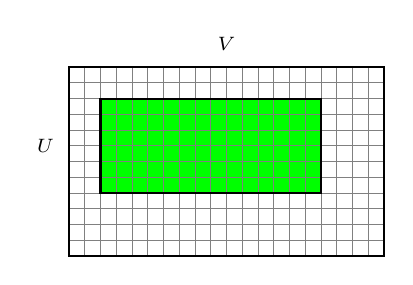
\begin{tikzpicture}
    \draw[fill = green] (0.4, -0.4) rectangle (3.2, -1.6);
    \draw[step = 0.2, gray, thin] (0, 0) grid (4, -2.4);
    \draw[black, thick] (0, 0) rectangle (4, -2.4);
    \draw[black, thick] (0.4, -0.4) rectangle (3.2, -1.6);
    \node at (-0.3, -1.) {\scriptsize $U$};
    \node at (2, 0.3) {\scriptsize $V$};
\end{tikzpicture}

            \end{center}
        \end{column}

		\begin{column}{0.48\textwidth}
            \begin{center}
                Треугольники:
                \vspace{0.2cm}
                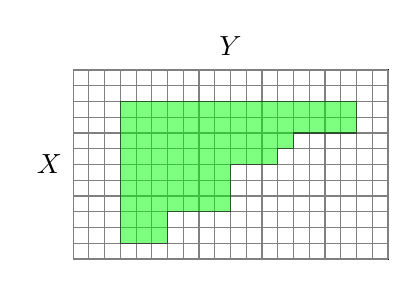
\begin{tikzpicture}
    \draw (0, 0) rectangle (4, -2.4);
    \draw[step = 0.2, gray, thin] (0, 0) grid (4, -2.4);
    
    \draw[fill = green, opacity = 0.5] (0.6, -0.4) -- (3.6, -0.4) -- (3.6, -0.8) -- (2.8, -0.8) -- (2.8, -1) --
    	(2.6, -1) -- (2.6, -1.2) -- (2, -1.2) -- (2, -1.8) -- (1.2, -1.8) -- (1.2, -2.2) -- (0.6, -2.2) --
        cycle;
    \node at (-0.3, -1.2) {$X$};
    \node at (2, 0.3) {$Y$};
\end{tikzpicture}

            \end{center}
		\end{column}
	\end{columns}
\end{frame}


\begin{frame}{$\KWm$ отношение (еще раз)}

    $f:\{0, 1\}^n \to \{0, 1\}$ монотонная частичная функция
    
    \begin{itemize}
        \item Алиса получает $x \in f^{-1}(1)$, Боб получает $y \in f^{-1}(0)$;
        \item цель~--- найти такую позицию $i \in [n]$, что $x_i = 1 \land y_i = 0$.
    \end{itemize}

    \pause

    \begin{theorem}[Разборов 95; Pudl{\'{a}}k 10; С 17]
        Для функции $f$ существует монотонная булева \alert{схема} размера $S$ тогда и только тогда, когда
        существует коммуникационный протокол \alert{на графе} для $\KWm_f$ размера $S$.
    \end{theorem}

    \pause

    \begin{theorem}[Hrube{\v{s}} Pudl{\'{a}}k 17]
        Для функции $f$ существует монотонная вещественная схема размера $S$ тогда и только тогда, когда
        существует коммуникационный протокол с треугольниками на графе для $\KWm_f$ размера $S$.
    \end{theorem}
\end{frame}


\begin{frame}{$\Search_{\varphi}$ (Lov{\'{a}}sz et al. 1994)}
    
    $\varphi(x, y)$~--- невыполнимая формула в КНФ:
    \begin{itemize}
        \item Алиса получает подстановку переменным $x$, Боб получает подстановку переменным $y$;
        \item цель~--- найти клоз $C \in \varphi$, который не выполнен подстановкой.
    \end{itemize}

    \pause

    \begin{theorem}[Kraj{\'{\i}}{\v{c}}ek 95; С 17]
        $CC_{\log(n)}$-доказательство формулы $\varphi$ размера $S$ $\Rightarrow$ протокол на графе
        размера $\poly(n) S$ для $\Search_{\varphi}$.
    \end{theorem}

    Резолюция, $\CP^*$, $\dots$~--- $CC_{\log(n)}$ системы доказательств.

    \pause
    
    \begin{theorem}[S 17]
        $\CP$-доказательство формулы $\varphi$ размера $S$ $\Rightarrow$ протокол с треугольниками на
        графе размера $S$ для $\Search_{\varphi}$.
    \end{theorem}
\end{frame}